
\subsection{Thermodynamical quantities}
\begin{frame}{Thermodynamical quantities}
	\centering
	Following, we are going to present physical quantities for both spin systems.\\[1em]
\end{frame}

%%%%%%%%%%%%%%%%%%%%%%%%%%%%%%%%%%%%%%%%
%%%%%%%%%%%%%%%%%%%%%%%%%%%%%%%%%%%%%%%%

\begin{frame}{Entropy}{\phantom{ }}
\onslide<+->{%
Shannon entropy for a system is defined by 
\begin{equation}
    S = -\k D\sum_{s\,\in\,\text{states}} p^{s} \ln p^{s},\label{eq:S_shann}
\end{equation}
where $D$ is the total number of spins and $p^{s}$ are the probabilities of finding a spin on a state $s$.}
\onslide<+->{%
\begin{itemize}
	\item For links:
\begin{equation}
    \label{eq:Sl}
	S_\ell  = - \k L \Big[ p_\ell^+\ln(p_\ell^+) + p_\ell^-\ln(p_\ell^-) \Big], 
\end{equation}
	\item For triangles:
\begin{equation}
    S_t = - \k C \left[ p_t^+\ln(p_t^+) + p_t^-\ln(p_t^-) \right], \label{eq:St}
\end{equation}}
\end{itemize}
\onslide<+>{%
Also, average entropies will be defined:
\begin{itemize}
	\item For links:
\begin{equation}
    \label{eq:sl}
	s_\ell  = \frac{S_\ell}{L}
\end{equation}
	\item For triangles:
\begin{equation}
	\label{eq:st}
    s_t = \frac{S_t}{C}
\end{equation}
\end{itemize}}

\end{frame}
%%%%%%%%%%%%%%%%%%%%%%%%%%%%%%%%%%%%%%%%
%%%%%%%%%%%%%%%%%%%%%%%%%%%%%%%%%%%%%%%%

\begin{frame}{Results for link entropy}
\setlength\fboxsep{0pt}
\setlength\fboxrule{0pt}
\vspace{-2mm}
\begin{figure}[h]
 \centering
 \fbox{\adjincludegraphics[trim={{0.11\width} {0.135\height} {0.1\width} {0.184\height}},clip,height=0.8\textheight]{SE_plane}}
 \caption{\textbf{Link entropy} across different configurations on the configuration space. Plotted with $N=155$.}
 \label{fig:ps_sL}
\end{figure}
\end{frame}

\setlength\fboxsep{0pt}
\setlength\fboxrule{0pt}
\begin{frame}{Results for link entropy}
\vspace{-2mm}
\begin{figure}[h]
    \centering
    \fbox{%
    \adjincludegraphics[trim={{0.18\width} {0.135\height} {0.13\width} {0.184\height}},clip,height=0.8\textheight]{SE}}
    \caption{\textbf{Link entropy} plotted vertically against how many legislators have chosen each of two vote options. Plotted with $N=155.$}
    \label{fig:SL}
\end{figure}
\end{frame}

\begin{frame}[t]{Results for link entropy}{Critical points}
	\setlength\fboxrule{0.5pt}
	\setlength\fboxsep{4pt}
\fbox{\begin{minipage}{0.6\textwidth}
		Let's recall that
		$$s_\ell =  - \k \Big[ p_\ell^+\ln(p_\ell^+) + p_\ell^-\ln(p_\ell^-) \Big],$$
		$$		p_\ell^{+} = \frac{L^{+}}{L},\qquad\text{and}\qquad		L^{+} = \left( \frac{1}{2}\|\vec{n}\|^2 - \frac{N}{2}\right)$$
\end{minipage}}\\[1em]

We differentiate $s_\ell$ to get its critical points.
\begin{align}
	\frac{\p s_\ell }{\p n_i} &= \frac{\p s_\ell}{\p p^{+}} \frac{\p p^{+}}{\p n_i} = -\k \bigg[ \ln(p^{+}) - \ln(p^{-}) \bigg] \left[ \frac{\|\vec{n}\|}{L}  \frac{\p}{\p n_i} \|\vec{n}\|  \right] 
.\end{align}
\\[2em]

\begin{itemize}
	\item $\left[ \frac{\|\vec{n}\|}{L}  \frac{\p}{\p n_i} \|\vec{n}\|  \right] =0\qquad  \to \qquad \vec{n} = \{N / k, \ldots, N / k \}$ 
	\item $\Big[ \ln(p^{+}) - \ln(p^{-}) \Big] = 0 \qquad \to \qquad L^{+} = L^{-}$
\end{itemize}
	
\end{frame}

\begin{frame}{Results for link entropy}{Maximum for Link entropy}
We can get an expression for the points where $L^{+}=L^{-}$.
\begin{align*}
     0 &= L^{+} - L^{-} =  2 \left[ \sum_{i=1}^{k-1} n_i^2 + \left( N-\sum_{i=1}^{k-1} n_i \right)^2   \right]   - N(N +  1) 
.\end{align*}
\begin{minipage}[c]{0.44\textwidth}
For the specific case of $k=3$, this results on the curve\\
	\strut\vspace*{-\baselineskip}\newline
	\begin{equation}
		\begin{aligned}
		    \frac{N \left(N - 1\right)}{4} &=  N \left(n_{1} + n_{2}\right) \\
			&- n_{1} n_{2} \\
			& - n_{1}^{2} - n_{2}^{2}, \label{eq:Lp_eq_Lm}
		\end{aligned}
	\end{equation}
	which is plotted on \Cref{fig:Lp_eq_Lm}. \\

The drawn ellipsis is consistent with the maximum observed on \Cref{fig:SL}.
\end{minipage}
\hspace{4mm}
\begin{minipage}[c]{0.47\textwidth}
\strut\vspace*{-\baselineskip}\newline
\begin{center}
	\vspace{-5mm}
	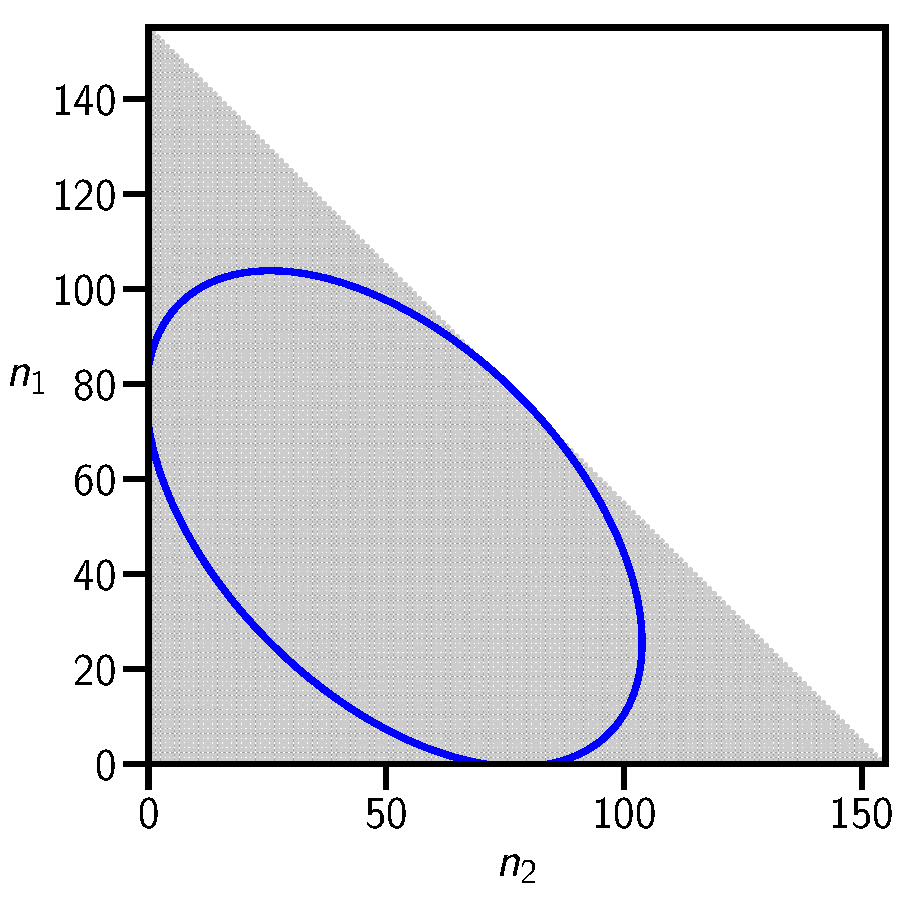
\includegraphics[width=1\linewidth]{elipse}
	\captionof{figure}{Subspace of the configuration space where link entropy is maximum. View from above.}
    \label{fig:Lp_eq_Lm}
\end{center}
\end{minipage}
\end{frame}

\begin{frame}{Results for triangle entropy}
\setlength\fboxsep{0pt}
\setlength\fboxrule{0pt}
\vspace{-2mm}
\begin{figure}[h]
 \centering
 \fbox{\adjincludegraphics[trim={{0.11\width} {0.135\height} {0.10\width} {0.184\height}},clip,height=0.8\textheight]{ST_plane.pdf}}
 \caption{\textbf{Triangle entropy} across different configurations on the configuration space. Plotted with $N=155.$}
 \label{fig:ps_sT}
\end{figure}
\end{frame}



%%%%%%%%%%%%%%%%%%%%%%%%%%%%%%%%%%%%%%%%
%%%%%%%%%%%%%%%%%%%%%%%%%%%%%%%%%%%%%%%%

\begin{frame}{Magnetizations}{\phantom{ }}
	\onslide<+->{
		We define two types of magnetizations. For the links we will have 
		\begin{equation}
			M_\ell  = L^+ - L^-= \|\vec{n}\|^2  - \frac{N(N+1)}{2}, 
			\label{eq:Ml}
		\end{equation}
		and another for the triangles 
		\begin{equation}
			M_t = C^+ - C^- = \frac{1}{6} \left[ 2N -4 \|\vec{n}\|^{3}_{3} + 6N \|\vec{n}\|^{2} -3N^2 - N^3  \right]. 
			\label{eq:Mt}
		\end{equation}
	}
	\onslide<+->{
		We also define their average counter parts as 
		\begin{equation}
			m_\ell  = \frac{M_\ell}{L},
			\label{eq:ml}
		\end{equation}
		and
		\begin{equation}
			m_t = \frac{M_t}{C}.
			\label{eq:mt}
		\end{equation}
	}
\end{frame}

%%%%%%%%%%%%%%%%%%%%%%%%%%%%%%%%%%%%%%%%
%%%%%%%%%%%%%%%%%%%%%%%%%%%%%%%%%%%%%%%%

\begin{frame}{Results for link magnetizations}
\vspace{-2mm}
 \begin{figure}[h]
	 \setlength\fboxsep{0pt}
	 \setlength\fboxrule{0pt}
     \centering
     \fbox{\adjincludegraphics[trim={{0.10\width} {0.13\height} {0.1\width} {0.18\height}},clip,height=0.80\textheight]{results-figs/magE_plane}}%
     \caption{\textbf{Link magnetization} across different configurations on the configuration space. Plotted with $N=155.$}
     \label{fig:ps_magL}
 \end{figure}%
\end{frame}

\begin{frame}{Results for triangle magnetization}
\vspace{-2mm}
 \begin{figure}[h]
	 \setlength\fboxsep{0pt}
	 \setlength\fboxrule{0pt}
     \centering
     \fbox{\adjincludegraphics[trim={{0.10\width} {0.13\height} {0.1\width} {0.18\height}},clip,height=0.8\textheight]{magT_plane}}
     \caption{\textbf{Triangle magnetization} across different configurations on the configuration space. Plotted with $N=155.$}
     \label{fig:ps_magT}
 \end{figure}
\end{frame}


%%%%%%%%%%%%%%%%%%%%%%%%%%%%%%%%%%%
%%%%%%%%%%%%%%%%%%%%%%%%%%%%%%%%%%%

	
\begin{frame}{Hamiltonian}
	We define the energy for the system in such way it is minimal when everyone agrees with each other. 
\begin{itemize}
	\item All links would be positive
	\item All its triangles would be balanced 
\end{itemize}

For this, for a single triangle $t$ we have defined the energy function $h$ as
\begin{equation}
    h(t) = - \sum_{\mathclap{\text{sides of $t$}}} \text{sign of the side} 
\end{equation}
which is the negative sum of their sides. This would lead us to
\begin{equation}
        h(+++) = -3,\qquad
		h(+--) = -1,\qquad
		h(---) = 3,
    \label{eq:h_types}
\end{equation}
for each triangle type.\\[1em]
\end{frame}

\begin{frame}{Hamiltonian}
 Then, the energy for the whole system would be the sum of $h(t)$ for all triangles, or
 \begin{equation}
	H =	\sum_{\mathclap{t\in\text{triangles}}} h(t).
 \end{equation}
Since the network is fully-connected, each link belong to $(N-2)$ triangles. And since we are summing all of them, our Hamiltonian results 
\begin{equation}
	H = -(N-2)M_\ell.\label{eq:H_M}
\end{equation}
\end{frame}

%%%%%%%%%

\begin{frame}{Temperature}{\phantom{ }}

Thermodynamical definition of temperature:
\begin{equation}
    \frac{1}{T} = \left( \frac{\partial S}{\partial U} \right)_{\,\mathclap{N}} \label{eq:T_def}
\end{equation}
where 
\begin{itemize}
	\item  $T$ is the temperature
	\item $S$ the entropy
	\item $N$ the number of particles
	\item and $U$ the internal energy.
\end{itemize}
In our case we would have

\begin{align}
    \frac{1}{T} &=  \frac{\partial S_\ell}{\partial H}  = \frac{\p S_\ell}{\p m_\ell} \frac{\p m_\ell}{\p H}
\end{align}
but we still need to relate entropy with magnetizations
\end{frame}

\begin{frame}{Temperature}{Relating entropy with magnetization}
Both type of  entropies can be written in terms of their respective magnetization, but here we will focus on the link entropy.\\[1em]

Since
\begin{align*}
	m_\ell &= p_{\ell}^{+} - p_{\ell}^{-},\qquad  p_{\ell}^{+} + p_{\ell}^{-} = 1\\
	%m_t &= p_{t}^{+} - p_{t}^{-},\qquad  p_{t}^{+} + p_{t}^{-} = 1,
\end{align*}
we can express the probabilities $p_{\ell}$ as
\begin{align*}
    p_\ell^{+} &= \frac{1}{2}(1+m_\ell), \quad p_\ell^{-} = \frac{1}{2}(1-m_\ell),%\label{eq:pl+-_m}\\
	%\\p_t^{+} &= \frac{1}{2}(1+m_t),\quad
%    p_t^{-} = \frac{1}{2}(1-m_t).%\label{eq:pt+-_m}
\end{align*}
Then, the link entropy result
\begin{equation}
        S_\ell = - L\,\k \Biggr[\left(\frac{1+m_\ell}{2}\right) \ln\left(\frac{1+m_\ell}{2}\right) + \left(\frac{1-m_\ell}{2}\right)\ln \left(\frac{1-m_\ell}{2}\right)\Biggr]\label{eq:Sl_m}.
\end{equation}
%and
%\begin{equation}
%        S_t = - C\,\k \Biggr[\left(\frac{1+m_t}{2}\right) \ln\left(\frac{1+m_t}{2}\right) + \left(\frac{1-m_t}{2}\right)\ln \left(\frac{1-m_t}{2}\right)\Biggr],\label{eq:St_m}
%\end{equation}
%for links and triangles, respectively. 
\end{frame}

\begin{frame}{Temperature}
Now we can solve for $T$ on 
\begin{align*}
    \frac{1}{T} &= \frac{\p S_\ell}{\p m_\ell} \frac{\p m_\ell}{\p H}.
\end{align*}

After solving both partial derivatives we get 
\begin{equation}
	T = (N-2)\frac{2}{\k}\left[\ln \left(\frac{1+m_\ell}{1-m_\ell}\right) \right]^{-1}\label{eq:T_final}
\end{equation}

\end{frame}

%%%%%

\begin{frame}{Results for the temperature}
\vspace{-1mm}
\begin{figure}[h]
    \centering
    \fbox{\adjincludegraphics[trim={{0.13\width} {0.12\height} {0.11\width} {0.17\height}},clip,height=0.78\textheight]{Tps}}%
	\vspace{-1mm}
    \caption{\textbf{Temperature} on top of the configuration space. Plotted with $N=155$ and $\k=1.$}
    \label{fig:Tps}
\end{figure}
\end{frame}

\begin{frame}{Results for the temperature}
\vspace{-1mm}
\begin{figure}[h]
    \centering
    \fbox{\adjincludegraphics[trim={{0.16\width} {0.125\height} {0.17\width} {0.12\height}},clip,height=0.78\textheight]{Tpos-neg}}%
	\vspace{-1mm}
    \caption{Sign of temperature on top of configuration space. Plotted with $N=155.$}
    \label{fig:Tpos-neg}
\end{figure}
\end{frame}


%%%%%%%%%%%%%%%%%%%%%%%%%%%%%%%%%%%
%%%%%%%%%%%%%%%%%%%%%%%%%%%%%%%%%%%

\begin{frame}{Results for the temperature}{Temperature and energy}
	\setlength\fboxrule{0.5pt}
	\setlength\fboxsep{4pt}
\fbox{\begin{minipage}{0.5\textwidth}
		Let's recall that
	\begin{align*}
		M_\ell &= L\,m_\ell\\
		H &= -(N-2)M_{\ell}\\
		T &= (N-2)\frac{2}{\k}\left[\ln \left(\frac{1+m_\ell}{1-m_\ell}\right) \right]^{-1}
	\end{align*}
\end{minipage}}\\[1em]

	If we isolate $m_\ell$ from the temperature expression, we get that 	
\begin{equation}
    m_\ell = \tanh \left(\frac{N-2}{\k T}\right).\label{eq:ml_of_T}
\end{equation}
Now, joining it with the expressions for $H$ and $M_\ell$, it yield us that
\begin{align}
    H = -(N-2)L\tanh \left(\frac{N-2}{\k T}\right). \label{eq:H_of_T}
\end{align}
\end{frame}

\begin{frame}{Results for the temperature}{Temperature and energy}
	\begin{figure}[h]
	    \centering
		\includegraphics[height=0.65\textheight]{T_H}
	    \caption{Hamiltonian against temperature, from \cref{eq:H_of_T} with $N=155$ and $\k=1$. $H$ is not defined of for $T=0$, but in the plot it was considered as zero for looking purposes.}
	    \label{fig:T_H_out}
	\end{figure}    
\end{frame}

%%%%%%%%%%%%%%%%%%%%%%%%%%%%%%%%%%
%%%%%%%%%%%%%%%%%%%%%%%%%%%%%%%%%%

